\chapter{Generative Adversarial Nets}
A strategy to generate images with less math than Variational Autoencoders.

The idea is to start with a random noise that is normally drawn from a unit Gaussian (or something similar) and we will pass it through a Generator network. The Generator network looks very much like the decoder on the autoencoder and spits fake images. Then, a discriminator network is responsible for deciding/estimating if the input image is fake or a real.

\begin{figure}[!htb]
  \centering
  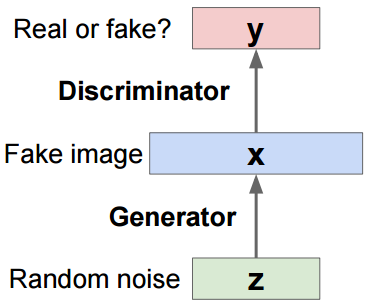
\includegraphics[width=0.25\textwidth]{Images/gans/8.png}
  \caption{GAN}
\end{figure}

\subsection*{How to we train them?}
\begin{figure}[!htb]
  \centering
  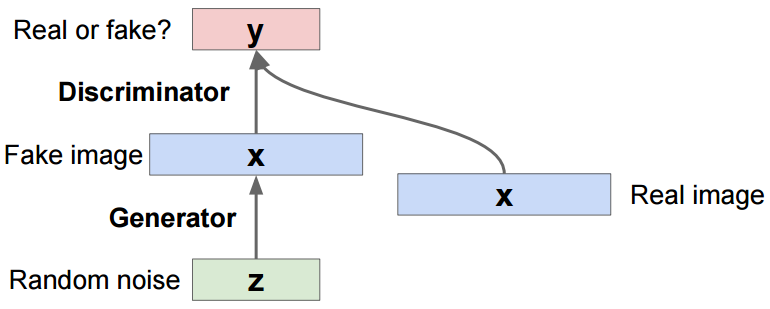
\includegraphics[width=0.5\textwidth]{Images/gans/7.png}
  \caption{GAN}
\end{figure}
We train this network all together. The Generator will receive minibatches of random noise, at it will spit fake images. The Discriminator will receive batches partially fake and real; and it will try to decide which ones are real and which ones are fake.

The generator will improve its fake images by trying to trick the discriminator.



\subsection*{Examples}
Interpolating random noise vectors. In figure \ref{fig:gans1} the images in the left and right extremes are obtained by sampling two random points (vectors) of the $z$ space and passing them through the generative net. Then the interpolation between pairs of extreme images is performed by interpolating the $z$ vectors and passing them through the generative net.
\begin{figure}[!htb]
  \centering
  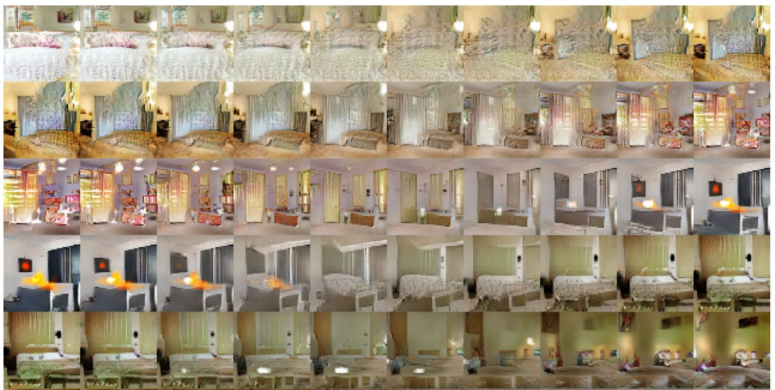
\includegraphics[width=0.6\textwidth]{Images/gans/9.png}
  \caption{Interpolating random noise vectors}
  \label{fig:gans1}
\end{figure}

Another experiment shows that the generator is learning a useful representation of the data. In this experiment they randomly generated multiple images of faces and then manually organized in the classes "smiling woman", "neutral woman", "neutral man". Then, they produce the mean $z$ average representation of each image and perform the arithmetic operation of z\_{smiling woman}-z\_{neutral woman}+z\_{neutral man} produces a smiling man.

\begin{figure}[!htb]
  \centering
  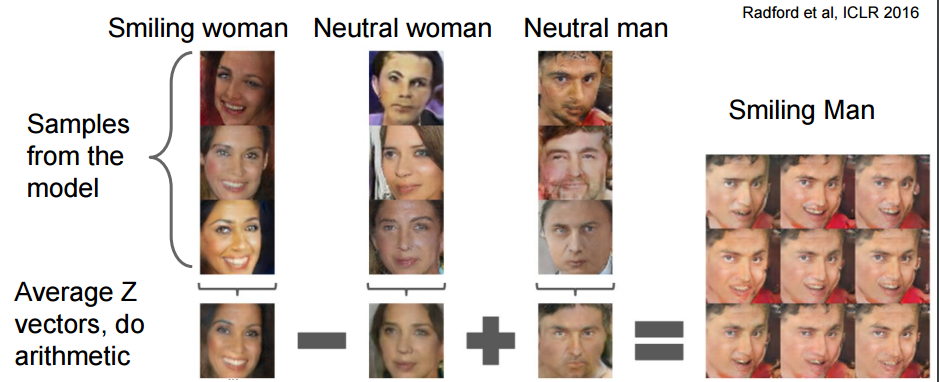
\includegraphics[width=0.6\textwidth]{Images/gans/10.png}
  \caption{Generator learning a useful representation of the data}
\end{figure}